\section{Base de Imagens} \label{pontosBaseImg}

Para a execução dos experimentos desta etapa do projeto será utilizada a base de imagens mostrada nas Figuras \ref{figBaseFrente}, \ref{figBaseDireita}, \ref{figBaseEsquerda}, \ref{figBaseCima} e \ref{figBaseBaixo}. Estas, por sua vez, registram um mesmo objeto em diferentes ângulos num ambiente que possui níveis de iluminção extremos. Para cada ângulo do objeto, foram registradas imagens em diferentes tempos de exposição, para que assim possam ser utilizadas pelos métodos de geração de imagens HDR, e então gerar a nuvem de pontos.

\begin{figure}[H]
  \centering 
  \subfloat[Tempo de exposição de $5.10^{-4}s$.]
  {
    \includegraphics[height=4cm]{BaseObjeto/Frente/1}
    \label{figBaseFrenteA}
  }
  \quad %espaco separador
  \subfloat[Tempo de exposição de $8.10^{-3}s$.]
  {
    \includegraphics[height=4cm]{BaseObjeto/Frente/2}
    \label{figBaseFrenteB}
  }
  \quad %espaco separador
  \subfloat[Tempo de exposição de $0,025s$.]
  {
    \includegraphics[height=4cm]{BaseObjeto/Frente/3}
    \label{figBaseFrenteC}
  }
  \quad %espaco separador
  \subfloat[Tempo de exposição de $0,1s$.]
  {
    \includegraphics[height=4cm]{BaseObjeto/Frente/4}
    \label{figBaseFrenteD}
  }
  \caption{Registro em diferentes tempos de exposição da frente do objeto.}
  \label{figBaseFrente}
\end{figure}

\begin{figure}[H]
  \centering 
  \subfloat[Tempo de exposição de ${1,56}.10^{-3}s$.]
  {
    \includegraphics[height=4cm]{BaseObjeto/Direita/1}
    \label{figBaseDireitaA}
  }
  \quad %espaco separador
  \subfloat[Tempo de exposição de $2,5.10^{-3}s$.]
  {
    \includegraphics[height=4cm]{BaseObjeto/Direita/2}
    \label{figBaseDireitaB}
  }
  \quad %espaco separador
  \subfloat[Tempo de exposição de $6,25.10^{-3}s$.]
  {
    \includegraphics[height=4cm]{BaseObjeto/Direita/3}
    \label{figBaseDireitaC}
  }
  \quad %espaco separador
  \subfloat[Tempo de exposição de $0,033s$.]
  {
    \includegraphics[height=4cm]{BaseObjeto/Direita/4}
    \label{figBaseDireitaD}
  }
  \caption{Registro em diferentes tempos de exposição da esquerda do objeto.}
  \label{figBaseDireita}
\end{figure}

\begin{figure}[H]
  \centering 
  \subfloat[Tempo de exposição de ${1,56}.10^{-3}s$.]
  {
    \includegraphics[height=4cm]{BaseObjeto/Esquerda/1}
    \label{figBaseEsquerdaA}
  }
  \quad %espaco separador
  \subfloat[Tempo de exposição de $5.10^{-3}s$.]
  {
    \includegraphics[height=4cm]{BaseObjeto/Esquerda/2}
    \label{figBaseEsquerdaB}
  }
  \quad %espaco separador
  \subfloat[Tempo de exposição de $0,016s$.]
  {
    \includegraphics[height=4cm]{BaseObjeto/Esquerda/3}
    \label{figBaseEsquerdaC}
  }
  \quad %espaco separador
  \subfloat[Tempo de exposição de $0,05s$.]
  {
    \includegraphics[height=4cm]{BaseObjeto/Esquerda/4}
    \label{figBaseEsquerdaD}
  }
  \caption{Registro em diferentes tempos de exposição da direita do objeto.}
  \label{figBaseEsquerda}
\end{figure}

\begin{figure}[H]
  \centering 
  \subfloat[Tempo de exposição de ${2,5}.10^{-3}s$.]
  {
    \includegraphics[height=4cm]{BaseObjeto/Cima/1}
    \label{figBaseCimaA}
  }
  \quad %espaco separador
  \subfloat[Tempo de exposição de $0,01s$.]
  {
    \includegraphics[height=4cm]{BaseObjeto/Cima/2}
    \label{figBaseCimaB}
  }
  \quad %espaco separador
  \subfloat[Tempo de exposição de $0,04s$.]
  {
    \includegraphics[height=4cm]{BaseObjeto/Cima/3}
    \label{figBaseCimaC}
  }
  \caption{Registro em diferentes tempos de exposição da parte de cima do objeto.}
  \label{figBaseCima}
\end{figure}

\begin{figure}[H]
  \centering 
  \subfloat[Tempo de exposição de ${2,5}.10^{-3}s$.]
  {
    \includegraphics[height=4cm]{BaseObjeto/Baixo/1}
    \label{figBaseBaixoA}
  }
  \quad %espaco separador
  \subfloat[Tempo de exposição de $6,25.10^{-3}s$.]
  {
    \includegraphics[height=4cm]{BaseObjeto/Baixo/2}
    \label{figBaseBaixoB}
  }
  \quad %espaco separador
  \subfloat[Tempo de exposição de $0,02s$.]
  {
    \includegraphics[height=4cm]{BaseObjeto/Baixo/3}
    \label{figBaseBaixoC}
  }  
  \quad %espaco separador
  \subfloat[Tempo de exposição de $0,1s$.]
  {
    \includegraphics[height=4cm]{BaseObjeto/Baixo/4}
    \label{figBaseBaixoD}
  }
  \caption{Registro em diferentes tempos de exposição do objeto visto por baixo.}
  \label{figBaseBaixo}
\end{figure}

Esta base de imagem será utilizada no processo proposto na Seção \ref{pontosProposta}. E para fins de comparação as Figuras \ref{figBaseFrenteB}, \ref{figBaseDireitaC}, \ref{figBaseEsquerdaC}, \ref{figBaseCimaC} e \ref{figBaseBaixoC}, serão utilizadas no método de obtenção de nuvem de pontos a partir de imagens LDR convencional. Estas foram escolhidas por serem avaliadas visualmente como sendo as mais bem expostas de cada ângulo registrado.